\documentclass[12pt]{report}
\usepackage{graphicx}
\usepackage{geometry}
\usepackage{float}
\usepackage{subcaption}
\usepackage{setspace}
\usepackage{hyperref}
\usepackage[italian]{babel}
\usepackage{verbatim}
\usepackage{biblatex}
\usepackage[nottoc]{tocbibind}

\addbibresource{thesis.bib}
\geometry{a4paper, bottom=5cm, left=4.2cm, right=4.2cm, heightrounded=true, bindingoffset=5mm}
\flushbottom

\begin{document}
\captionsetup[table]{name=Figura}

\newgeometry{margin=1in}
\begin{titlepage}


  \noindent
  \begin{minipage}[t]{0.19\textwidth}
    \vspace{-4mm}{
\includegraphics[scale=1.15]{img/logo_unimib.pdf}}
  \end{minipage}
  \begin{minipage}[t]{0.81\textwidth}
    {
      {\textsc{Università degli Studi di Milano - Bicocca}}\\
      \textbf{Scuola di Scienze}\\
      \textbf{Dipartimento di Informatica, Sistemistica e Comunicazione}\\
      \textbf{Corso di laurea in Informatica}\\
      \par
    }
  \end{minipage}

  \vspace{30mm}

  \begin{center}
    {\LARGE{
        \textbf{Simulated Annealing per l'inferenza di mutazioni ricorrenti in alberi tumorali}}}
  \end{center}

  \vspace{40mm}

  \noindent
  {\large \textbf{Relatore:} \textit{Prof. Gianluca Della Vedova} }

  \noindent
  {\large \textbf{Correlatore:} \textit{Dott. Simone Ciccolella}}

  \vspace{50mm}

  \begin{flushright}
    \textbf{\large Relazione della prova finale di:\\}
    \large{\textit{Stefano Giacomini}}\\
    \large{\textit{Matricola 829854}}
  \end{flushright}

  \vspace{15mm}
  \begin{center}
    {\large{\bf Anno Accademico 2020-2021}}
  \end{center}

  \restoregeometry

\end{titlepage}
\restoregeometry

\onehalfspacing
{\pagestyle{plain}
  \tableofcontents
  \cleardoublepage}

\chapter{Introduzione}

  Recenti sviluppi riguardanti la terapia mirata per la cura di tumori fanno affidamento su un'accurata inferenza della mutazione clonale e della progressione della malattia.
  Diversi studi\cite{Morrissy2016}\cite{Wang2016} sottolineano come capire l'ordine di accumulazione e la prevalenza delle mutazioni somatiche durante la progressione del tumore può aiutare a progettare meglio queste strategie di trattamento.\\\\
  La maggior parte delle tecniche correntemente utilizzate per l'inferenza di progressioni tumorali si basa su dati provenienti da esperimenti di sequenziamento di massa, dove solo una parte delle delle mutazioni osservabili da un grande numero di cellule è ottenuta, senza la distinzione di quali cellule le contengono.\\\\
  Negli ultimi anni sono stati sviluppati molti approcci computazionali per l'analisi di dati di sequenziamenti di massa con lo scopo di inferire la scomposizione di subcloni tumorali e ricostruire la filogenesi dei tumori (alberi evolutivi)\cite{Bonizzoni227801}.\\\\
  Il problema principale di questa tecnica è che un campione ottenuto da un sequenziamento di massa contiene un misto sia di cellule sane che di cellule tumorali, e questa mutazione clonale può essere solo stimata dalla porzione di mutazioni osservate.\\\\
  Il sequenziamento a singola cellula, o \emph{SCS} (single-cell sequencing), promette di creare la migliore soluzione per capire la causa della progressione del tumore.
  Tuttavia la mancanza di accuratezza, riflessa nell'alta probabilità di falso positivo e nell'alto drop-out allelico, inerente alla tecnologia usata richiede l'uso di metodi che sono in grado di creare inferenze di progressioni tumorali dai dati prodotti dalle correnti tecniche di \emph{SCS}.\\\\
  Vari metodi sono stati recentemente sviluppati con questo scopo, molti di questi metodi però si basano sull'\emph{ISA} (Infinite Site Assumption), il quale essenzialmente indica come una mutazione possa essere acquisita al massimo una volta e mai essere persa.
  Un motivo per cui questo viene fatto è che questa assunzione semplificativa porta ad un modello evolutivo il cui problema è risolvibile da un algoritmo in tempo polinomiale, ovvero il modello di filogenesi perfetta\cite{gusfield1991efficient}.\\\\
  Questo metodo è sicuro da usare solo in determinate situazioni, come ad esempio l'evoluzione di una popolazione, dove tende ad essere la norma più che un eccezzione\cite{10.1093/genetics/61.4.893}.
  La progressione di cellule tumorali è però invece una situazione piuttosto estrema, dove le cellule sono sotto attacco del sistema immunitario, l'evoluzione è molto veloce e con un'alta probabilità di mutazione.\\\\
  Come risultato studi su dati prodotti da SCS stanno cominciando a rilevare fenomeni non spiegabili da un modello di filogenesi perfetta\cite{Kuipers2022.01.28.478229}\cite{Brown2017}.
  In questo lavoro utilizziamo quindi un modello Car-($k, r$), il quale è un modello più generale rispetto al modello di filogenesi perfetta, per permmettere la perdita e la ricorrenza di mutazioni.
  Una volta che però ci allontaniamo dal modello ideale di filogenesi perfetta\cite{gusfield1991efficient}, privo dalla possibilità di errori, passiamo ad un problema NP-hard.\\\\
  In più, la maggior parte dei metodi attualmente disponibili assumono che la probabilità di falso negativo sia la stessa per tutte le mutazioni.
  Se questa assunzione è valida per dati provenienti da campioni di DNA, la probabilità di falso negativo in campioni provenienti da RNA può variare a causa dei differenti livelli di espressione genetica.\\\\
  Visto che il nostro approccio è pensato per dati provenienti sia da DNA che da RNA i parametri passati possono essere settati per adattarsi a dati provenienti da uno piuttosto che dall'altro, permettendo quindi anche una probabilità di falso negativo diversa per ogni mutazione.\\\\
  Partendo dal metodo SASC\cite{10.1093/bioinformatics/btaa722}, un metodo di ricerca di filogenesi che massimizza la likelihood permettendo perdita di mutazioni incorporando il modello di Dollo\cite{10.2307/2412867}, abbiamo quindi sviluppato un metodo più generico.

  \section{Motivazioni}

  L'utilizzo di un modello più generico, che comprende anche mutazioni ricorrenti, diventa particolarmente importante quanto si deve descrivere l'evoluzione virale.\\\\
  Facendo un esempio molto attuale, il virus SARS-CoV-2, virus che è causa della malattia comunemente chiamata COVID-19, sono state riscontrate 198 mutazioni ricorrenti, la maggior parte delle quali hanno portato a cambiamenti a livello proteico\cite{VANDORP2020104351}.
  \'E importante lo studio di mutazioni che sono emerse indipendentemente più volte (omoplasia) in quanto sono molto probabilmente adattamenti del virus all'ospite, in questo caso quindi indicano l'adattamento del virus SARS-CoV-2 al genere umano\cite{VANDORP2020104351}.\\\\
  Per descrivere meglio anche questi casi è stato quindi sviluppato il metodo di Simulated Annealing per l'inferenza di mutazioni ricorrenti (o recurrent SASC), il quale permette sia la perdita che la ricorrenza di mutazioni, incorporando un modello Car-($k, r$).

\chapter{Definizioni}

\section{Problemi di ricostruzione di alberi filogenetici}
  Prima di cominciare a parlare del recurrent SASC vero e proprio è bene definire i concetti che verranno utilizzati.\\

  Un albero filogenetico è un grafico che mostra visivamente la collocazione temporale della separazione fra le linee evolutive che a partire da una data specie ha portato alla formazione di due o più specie diverse attraverso una serie di biforcazioni.
  Con filogenesi basata su caratteri, dove con carattere si intende una qualunque caratteristica che si può osservare, si intende quella filogenesi che sfrutta alcuni caratteri specifici, un esempio può essere la presenza o meno della colonna vertebrale, per rappresentare la storia evolutiva di alcune specie.\\\\
  Utilizzando questo concetto e applicandolo, invece che alla separazione di due linee evolutive dovuta ad una serie di mutazioni, all'acquisizione di una cellula di una determinata mutazione, si può rappresentare l'evoluzione di cellule tumorali.\\\\
  Come menzionato precedentemente la ricostruzione della progressione evolutiva di cellule tumorali può essere modellato con la costruzione di una filogenesi incompleta basata sui caratteri, dove ogni carattere rappresenta una mutazione.\\\\
  Consideriamo quindi come input una matrice  ${I}_{ij}$ di dimensioni $n$ x $m$, con $n$ numero delle cellule e $m$ numero delle mutazioni, e dove ${I}_{ij} = 0$ indica che la sequenza $i$ non ha la mutazione $j$, ${I}_{ij} = 1$ indica la presenza della mutazione $j$ nella sequenza $i$ e ? indica che non ci sono abbastanza informazioni sulla presenza/assenza di una mutazione $j$ nella sequenza $i$.
  Questa incertezza sulla presenza di una mutazione deriva da una insufficiente precisione nel sequenziamento del DNA/RNA.\\\\
  Oltre a questo ci sono altri problemi derivanti dal sequenziamento, infatti i valori della matrice di input possono anche contenere falsi positivi e falsi negativi, mentre la probabilità di falso positivo è in genere abbastanza bassa, la probabilità di falso negativo può essere alta e variare da una mutazioni all'altra.\\\\
  Quindi, detta $E_{ij}$ la matrice $n$ x $m$ di output finale, ovvero la matrice binaria senza errori o rumore prodotto dall'algoritmo, allora ${\alpha}_{j}$ indica la probabilità di falso negativo della mutazione $j$, mentre invece $\beta$ indica la probabilità di falso positivo.\\
  Di conseguenza, per ogni valore di ${E}_{ij}$, valgono le seguenti:
  \[
    P(I_{ij} = 0|{E}_{ij} = 0) = 1 - \beta P(I_{ij} = 0|E_{ij} = 1) = \alpha_{j}
  \]
  \[
    P(I_{ij} = 1|E_{ij} = 0) = \beta P(I_{ij} = 1|E_{ij} = 1) = 1 - \alpha_{j}
  \]
  Puntiamo quindi a trovare una matrice che massimizzi la likelihood della matrice osservata $I$ sotto la probabilità di falso negativo/positivo e i valori mancanti.\\\\
  Il nostro lavoro contiene in più la perdita di mutazioni e la possibilità di avere più ricorrenze della stessa mutazione, andiamo quindi a definire $P(L(j))={\gamma}_{j}$ come la probabilità di perdità della mutazione $j$ e il set di variabili ${c}_{j}$ per $j=1,...,m$ che denota il numero totale di perdite per la mutazione $j$ nell'albero.
  Definiamo poi $P(D(j))={\delta}_{j}$ come la probabilità di creare una copia della mutazione $j$ e il set di variabili ${f}_{j}$ per $j=1,...,m$ che denota il numero totale di copie per la mutazione $j$ presenti nell'albero.\\\\
  Un albero filogenetico $T$ di un set $C$ di $m$ mutazioni e $n$ cellule (affette da queste mutazioni) è definito come un albero con radice i cui nodi interni sono etichettati con le mutazioni di $C$, mentre le foglie sono etichettate dalle cellule.
  \'E importante far notare come l'etichettamento dei nodi deve rispettare alcune restrizioni a seconda del modello evolutivo che stiamo considerando. Per esempio, in una filogenesi perfetta, non possono esistere due nodi con la stessa etichetta.\\\\
  Questa è un'alternativa della classica filogenesi basata su caratteri, dove l'albero $T$ è definito come un set di caratteri e dove le foglie non hanno nessuna etichetta e rappresentano specie differenti.\\\\
  Lo \emph{stato} di un nodo $x$ è definito come il set di mutazioni acquisite ma non perse nel percorso dalla radice a $x$. Lo stato di ogni foglia $l$ di $T$ è rappresentato da un vettore binario di lunghezza $m$, chiamato profilo del genotipo, che denotiamo come $D(T, l)$, dove $D{(T, l)}_{j}=1$ se e solo se la foglia $l$ ha la mutazione $j$ e 0 altrimenti.\\\\
  Diciamo che l'albero $T$ \emph{codifica} una matrice $E$ se esiste una mappatura $\sigma$ delle righe (cellule) di $E$ nelle foglie di $T$ tale che $E_{i}=D(T, \sigma)_{i}$ per ogni riga $i$ di $E$, dove ${\sigma}_{i}$ denota l'immagine di una riga $i$ attraverso la mappatura $\sigma$.
  Detto in maniera meno formale, ${\sigma}_{i}$ è il nodo dell'albero filogenetico corrispondente al nodo a cui la cellula $i$ è attaccata.\\\\
  Notare come la matrice $E$ è completamente caratterizzata dalla coppia $D(T, \sigma)$.
  Dunque il nostro problema può essere espresso come trovare l'albero $T$ che massimizzi la seguente funzione obiettivo:
  \[
    \max{\sum_{j}^{m}[-c_{j}\log(1-P(L(j)))-f_{j}\log(1-P(D(j)))+\sum_{i}^{n}\log(P(I_{ij}|D(T, \sigma_{i})_{j}))]}
  \]
  Facciamo inoltre notare come i valori assegnati alle entrate sconosciute della matrice di input non contano nel calcolo della funzione obiettivo, ovvero $P(I_{ij}=\ ?|E_{ij}=1)=P(I_{ij}=\ ?|E_{ij}=0)$. Per semplificare il calcolo della likelihood supponiamo che $P(I_{ij}=\ ?|E_{ij}=1)=P(I_{ij}=\ ?|E_{ij}=0)=1$.
  In più $\sigma$ può essere computato direttamente da $T$, lasciando quindi $T$ come unica variabile da ottimizzare.

\section{Dollo-k e Camin-Sokal-k}
  Il modello di Dollo\cite{10.2307/2412867} assume che in filogenesi ogni singola mutazione è introdotta una sola volta nella storia evolutiva, ma che invece perdite della stessa possono occorrere un numero infinito di volte.
  Una restrizione di questo modello è ottenibile limitando il numero di perdide per ogni mutazione.\\\\
  Chiamiamo quindi Dollo-$k$ il modello evolutivo in cui ogni mutazione può essere acquisita solo una volta e persa al massimo $k$ volte.
  I casi speciali Dollo-0 e Dollo-1 corrispondono rispettivamente ai modelli di perfetta\cite{gusfield1991efficient} e persistente\cite{BONIZZONI201251} filogenesi.\\\\
  Invece il modello di Camin-Sokal\cite{https://doi.org/10.1111/j.1558-5646.1965.tb01722.x} permette molteplici occorrenze della stessa mutazione ma nessuna perdita.
  Definiamo quindi Camin-Sokal-$k$ il modello evolutivo in cui una mutazione può avere al più $k$ ripetizioni e non può mai essere persa. Il caso speciale Camin-Sokal-1 corrisponde al modello di filogenesi perfetta\cite{gusfield1991efficient}.\\\\
  Il modello utilizzato in questo lavoro è il Car-($k, r$), un modello che va ad unire i modelli introdotti precedentemente e che quindi ammette al massimo $k$ perdite (o backmutation) e $r$ ripetizioni (o recurrent mutation).
  Dove i modelli di filogenesi perfetta\cite{gusfield1991efficient} e filogenesi persistente\cite{BONIZZONI201251} si ottengono rispettivamente con i casi Car-(0, 1) e Car(1, 1).
  Il problema di ricorstruzione della filogenesi su un modello Car-($k, r$) è NP-completo\cite{GOLDBERG1996111} per ogni $k$ $>$ 1 e $r$ $>$ 0.\\\\
  Visto che il modello Car-(k, r) utilizza sia backmutation che recurrent mutation introduciamo due nuovi tipi di nodi nell'albero filogenetico, per esprimere le perdite e le ripetizioni delle mutazioni. Per ogni mutazione $p$ creiamo $k$ nuove mutazioni ${p^-}_{l}$ per ogni $l\in\{i, ..., k\}$, rappresentanti le possibili perdite della mutazione $p$, in più creiamo $r$ nuove mutazioni ${p}_{j}$ per ogni $j\in\{i, ..., r\}$ reppresentanto le possibili copie della mutazione $p$.\\\\
  In più imponiamo le due seguenti nuove regole:
  \begin{itemize}
    \item ogni nodo etichettato da una perdita di una mutazione $p^-$ debba essere discendente di un nodo etichettato dall'acquisizione di una mutazione $p$

    \item ogni nodo etichettato da $p$ non possa essere discendente di un'altro nodo etichettato con $p$, a meno che questo non sia prima stato perso con un nodo $p^-$
  \end{itemize}
  \'E importante sottolineare come, a differenza del modello a filogenesi perfetta, con l'introduzione di perdite e ricorrenze potremmo avere più alberi che sono soluzione del problema.

  \subsection{Modello utilizzato}
  Nel modello utilizzato sono state in più aggiunte le seguenti restrizioni: il numero massimo di perdite nell'intero albero è al massimo $d$ e il numero di copie è al massimo $z$.\\\\
  Questo fa si che la variabile $c$ sia soggetta a (i) ${c}_{j}\geq k \ \forall j$ e (ii) $\sum_{j}^m {c}_{j} \geq d$ e che in maniera analoga la variabile $f$ sia soggetta a (i) ${f}_{j}\geq r \ \forall j$ e (ii) $\sum_{j}^m {f}_{j} \geq z$.
  %\'E inoltre importante notare come con un numero di mutazioni $m$ abbastanza piccolo, settare la variabile $d$ con un valore abbastanza piccolo, per esempio 5, equivale a settare $k\leq 1$, rendendo quindi il valore di k irrilevante; un discorso analogo può essere fatto per quanto riguarda $r$ e $z$.

  \begin{table}[H]
    \begin{minipage}{0.45\textwidth}
    \centering
    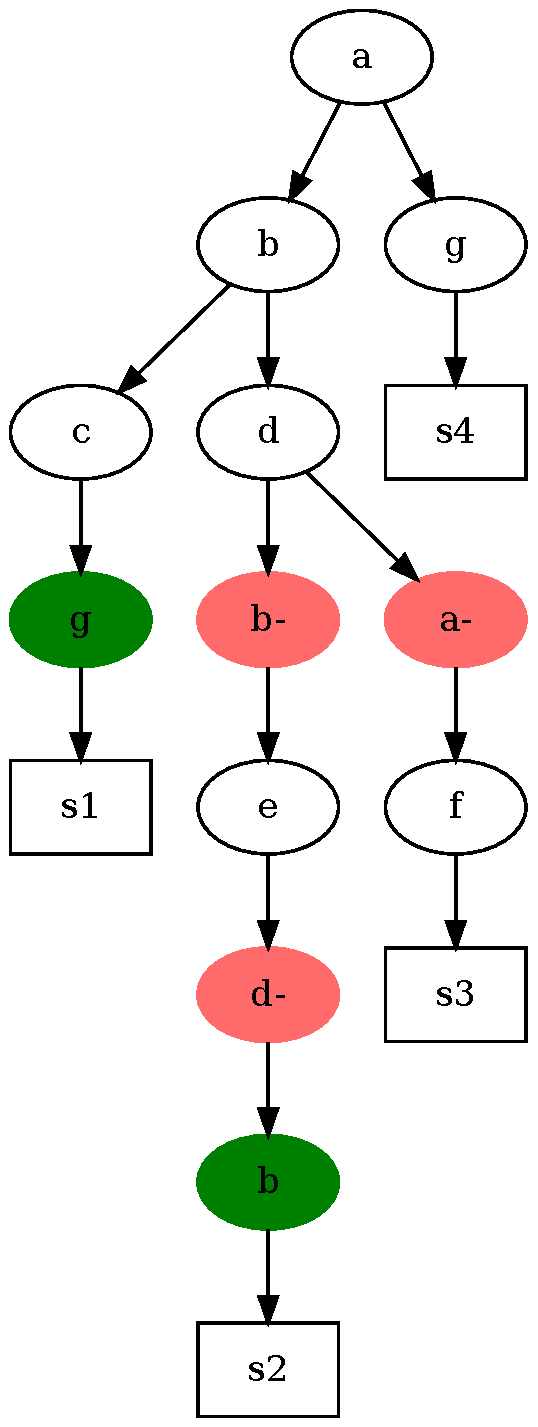
\includegraphics[scale = 0.33]{img/tree.pdf}
    \end{minipage}
    \begin{minipage}{0.5\textwidth}
    \centering
      \begin{tabular}{|l|l|l|l|l|l|l|l|}
        \hline
         & a & b & c & d & e & f & g\\
        \hline
        $s_{1}$ & 1 & 1 & 1 & 0 & 0 & 0 & 1\\
        \hline
        $s_{2}$ & 1 & 1 & 0 & 0 & 1 & 0 & 0\\
        \hline
        $s_{3}$ & 0 & 1 & 0 & 1 & 0 & 1 & 0\\
        \hline
        $s_{4}$ & 1 & 0 & 0 & 0 & 0 & 0 & 1\\
        \hline
      \end{tabular}
    \end{minipage}
    \caption{Esempio di una matrice $E$ (n=4, m=7), a destra, che esprime le cellule $\{ s_{1},...,s_{4}\}$ aventi il set $C = \{ a,...,g\}$ di mutazioni. L'albero $T$, a sinistra, è un albero di filogenesi di cellule tumorali raffigurante la matrice $E$,
    nel quale i nodi rappresentanti le backmutation sono colorati di rosso e i quelli rappresentanti le recurrent mutation sono colorati di verde. \'E importante far notare che la matrice non permette una filogenesi perfetta e che $T$ è una filogenesi Car-(1, 1)}
    \label{fig:fig1}
  \end{table}

\section{Simulated Annealing}
  Il fatto che ${c}_{j}\geq k \ \forall j$ e $\sum_{j}^m {c}_{j} \geq d$ e che ${f}_{j}\geq r \ \forall j$ e $\sum_{j}^m {f}_{j} \geq z$, e il fatto che vogliamo cercare l'albero che massimizzi la likelihood, rendono il problema di riscostruzione della filogenesi computazionalmente NP-hard sotto il modello Car($k$, $r$) per ogni $k > 0$ e $r > 0$. Per questo motivo si è deciso di utilizzare il metodo del Simulated Annealing\cite{Kirkpatrick1983} (SA) per cercare l'albero che massimizzi la likelihood di una determinata matrice di input, soddisfacendo il modello Car($k$, $r$), dove $k$ e $r$ sono dati come input.\\\\
  SA è una metaeuristica che sfrutta un metodo di ricerca randomico per esplorare la regione delle soluzioni ammissibili alla ricerca dell'ottimo, esattamente come tutte le altre metaeuristiche non c'è certezza che SA trovi la soluzione ottima della funzione obiettivo in un numero finito di step.\\\\
  SA è però in grado, rispetto ad altri metodi deterministici, di evitare di rimanere bloccato in ottimi locali in quanto può accettare anche step non migliorativi; nello specifico sia data $X_{c}$, soluzione di partenza dell'algoritmo, calcolo $X_{n}$, punto nell'intorno di $X_{c}$ calcolato da una mossa randomica, se $\Delta Z\geq0$, differenza dei valori della funzione obiettievo nei due punti, allora la nuova soluzione viene accetata e diventa la soluzione di partenza del prossimo step dell'algoritmo.\\\\
  Se invece $\Delta Z < 0$ ho comunque una probabilità che venga accetata ed è pari a: $e^{\frac{\Delta Z}{T}}$.
  Con $T$ che è una variabile chiamata \emph{temperatura} scelta inizialmente e che continua a diminuire nel tempo.\\\\
  Il metodo col quale si va diminuire la temperatura determina quanto velocemente raggiungiamo la soluzione finale e con quale complessità computazionale, il metodo utilizzato in questo lavoro è la riduzione geometrica della temperatura per cui vale la formula $T_{i}=(1-cooling\_rate)T_{i-1}$, dove il cooling rate è il tasso di riduzione della temperatura ad ogni passo.\\\\
  Come si può intuire dalla formula, una temperatura alta indica una più alta probabilità di accettare mosse molto peggiorative, favorendo l'\emph{exploration}, ovvero la ricerca all'interno della funzione per evitare di rimanere incastrati in ottimi locali, invece man mano che la temperatura diminuisce anche la probabilità di accettare mosse molto peggiorative, favorendo quindi l'\emph{exploitation}, ovvero la ricerca dell'ottimo nell'intorno in cui mi trovo, con $T\approx 0$ non accetto più soluzioni peggiorative.
  Il criterio di arresto dell'algoritmo in genere è il raggiungimento della $T$ minima, scelta inizialmente.

\chapter{Metodo}
  Si discute ora il metodo col quale si ricostruisce l'albero evolutivo massimizzando la \emph{likelihood}, ovvero il valore che indica la bontà della soluzione trovata.\\\\
  A tal fine sono state fatte diverse aggiunte alla codebase di \textbf{SASC} e quindi è bene, come prima cosa, analizzare le strumentazioni, ovvero il linguaggio di programmazione e le librerie principali, usate nel progetto.

  \section{Introduzione agli strumenti utilizzati}
  \subsection{Librerie e linguaggio}

  Nel progetto è stato utlizzato come linguaggio \emph{C}, ai fini del progetto non sono stati aggiunti nuovi file sorgenti ma sono state fatte aggiunte e modifiche all'interno della \textit{codebase}.\\\\
  Bisogna, quindi, citare una serie di librerie esterne utilizzate in diverse parti del codice C:
  \begin{itemize}
    \item La libreria \textbf{vector}, che permette l'implementazione della struttura dati dei \textit{vettori} nel linuaggio \textit{C}

    \item La libreria \textbf{tree}, che permette l'implementazione di nodi etichettati di alberi evolutivi nel linguaggio \textit{C}, rapprentando anche backmutation e recurrent mutation

    \item La libreria \textbf{mt19937ar}\cite{mt19937ar}, che consente di generare numeri casuali in vari maniere, nello specifico nel progetto viene utilizza per generare numeri casuali all'interno di determinati range o per generare unsigned int a 32-bit casuali
  \end{itemize}

  \subsection{Graphviz}
  Un altro strumento utlizzato è stato sotware open source per la visualizzazzione di grafi \textbf{Graphviz}\cite{graphviz}, che, data la descrizione di un grafo, ne crea il diagramma in vari formati quali, per esempio pdf o SVG.\\\\
  La descrizione del grafo da creare può essere passata o direttamente nel terminale o attraverso un file con estensione \emph{GV}.
  I file \emph{GV} contengono descrizioni riguardanti grafi scritte nel linguaggio \emph{DOT}, il quale è un linguaggio per la rappresentazione di grafi che può essere interpretato da Graphviz o da altri programmi che lo usano internamente.\\\\
  Nel linguaggio DOT un grafico inizia con una direttiva che indica se il grafo è un grafo orientato (\textbf{digraph}) o un grafo non orientato (\textbf{graph}), semanticamente, questo indica se c'è o meno una direzione nell'arco che collega due nodi.\\\\
  Opzionalmente, un grafo può anche essere descritto come \textbf{strict}, questa opzione rende impossibile la creazione di nodi multipli, ovvero ci può essere al massimo un arco che va da un determinato nodo di partenza ad un determinato nodo di arrivo, nel caso di un grafo orientato, invece nel caso sia un grafo non orientato significa che ci può essere al massimo un arco che connete due nodi.\\\\
  Può in più, in maniera opzionale, venire assegnato un ID al grafo, in seguito tra due parentesi graffe viene decritto il corpo del grafo, nel quale vengono descritti i nodi e gli archi (\textbf{stmt\_list}). La struttura può essere riassunta come:
  \[[strict]\,\,(graph \,\,|\,\, digraph)\,\,[ID]\,\,\{stm\_list\} \]
  Nella stmt\_list possono essere passati sia attributi riguardanti il grafo (per esempio, dimensione del font) che attributi riguardanti i nodi e gli archi.\\\\
  Gli archi devono essere segnati come "$->$" nel caso abbia un grafo orientato e come "$--$" nel caso abbia un grafo non orientato.\\\\
  Graphviz possiede vari opzioni per quanto riguarda il colore e la forma dei nodi ma anche font, stili di archi e in generale altre opzioni per personalizzare l'estetica di un grafo.\\\\
  Il linguaggio DOT è stato utlizzato come output del codice sia per stampare sul terminale gli alberi creati che per creare un file GV di output contente l'albero migliore.
  Un esempio del linguaggio DOT è:
  \begin{small}
  \begin{verbatim}
  digraph boxes_and_circles {
    // a 'graph' statement
    graph [overlap = true, fontsize = 10]

    // several 'node' statements
    node [shape = box,
          fontname = Helvetica]
    A; B; C; D; E; F

    node [shape = circle,
          fixedsize = true,
          width = 0.9] // sets as circles
    1; 2; 3; 4; 5; 6; 7; 8

    // several 'edge' statements
    A->1 B->2 B->3 B->4 C->A
    1->D E->A 2->4 1->5 1->F
    E->6 4->6 5->7 6->7 3->8
  }
  \end{verbatim}
  \end{small}
  Il quale, attraverso Graphviz, crea il seguente albero:
  \begin{center}
  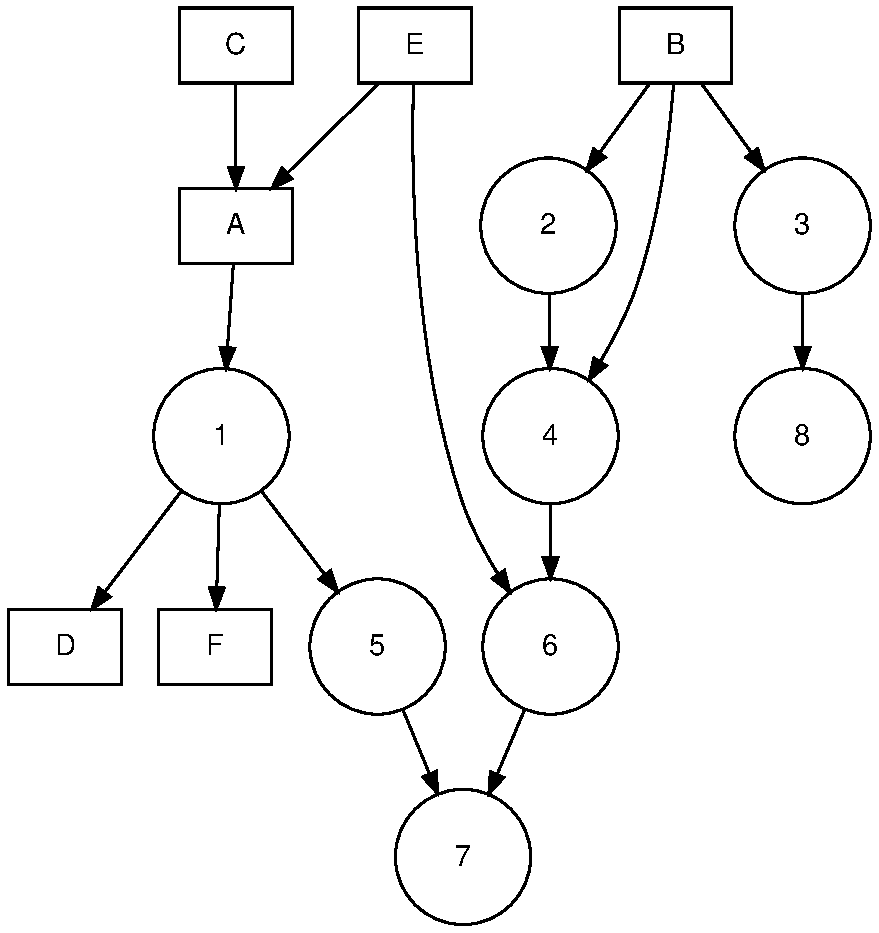
\includegraphics[scale = 0.4]{img/esempio.pdf}
  \end{center}

  \section{Input}
  Iniziamo quindi a descrivere come funziona il codice di \emph{recurrent SASC} vero e proprio.\\\\
  La prima parte riguarda ai dati di input che vengono passati, che ruguardano sia il modello utilizzato, Car-($k, r$), sia la matrice indicante le mutazioni delle varie cellule e in più anche i dati relativi a falso positivo e falso negativo.\\\\
  Riguardo al modello Car-($k, r$) vengono passati inanzitutto i valori $k$ e $r$ del modello, i quali indicano rispettivamente il numero massimo di backmutation e di recurrent mutation di ongi mutazione e $d$ e $z$ che sono il numero massimo di backmutation e recurrent mutation presenti nell'intero albero, questi ultimi dati se non vengono passati sono impostati +inf, le probabilità $\gamma$ e $\delta$, che sono le probabilità di aggiungere backmutation e recurrent mutation, le quali possono essere diverse per ogni mutazione (e quindi passate attraverso un file) o le stesse per ogni mutazione dell'albero.\\\\
  Per quanto riguarda invece la matrice di input invece vengono sia passati $n$ e $m$, numero di cellule e numero di mutazioni, che la matrice vera e propria rappresentata da un file di testo contente 1, 0, i quali indicano rispettivamente la presenza e la non presenza di una mutazione in una certa cellula, e 2, il quale indica che non ci sono abbastanza informazioni sulla presenza/assenza della mutazione in quella cellula (ciò che prima avevamo indicato con ?).\\\\
  Possono poi essere passati i dati riguardanti il Simulated Annealing, ovvero la temperatura iniziale e il cooling rate, il quale indica quanto velocemente la temperatura diminuisce nel tempo.

  \section{Calcolo likelihood}
  Prima di parlare della funzione che calcola la likelihood è bene introdurre brevemente come l'abero, le backmutation e le recurrent mutation vengono tenute in memoria e passate nelle varie funzioni che le utilizzano.\\\\
  Gli alberi vengono passati come un vettori di nodi dove ogni nodo contiene dati riguardanti: nodi figli, nodo padre, nodi "fratelli" e se il nodo è backmutation, recurrent mutation o un nodo normale.\\\\
  Le backmutation e le recurrent vengono passate ognuna da un proprio vettore contenete la posizione dei vari nodi particolari e un array di interi di dimensione m dove ogni elemento indica il numero di backmutation o recurrent mutation di quella mutazione. Esiste poi un array di int contenente l'id delle mutazioni "originali", dove con originali si intende nodi che non sono ne backmutation ne recurrent mutation.\\\\
  \begin{table}[H]
    \tiny
    \centering
    \begin{tabular}{|l|}
     \hline
     \multicolumn{1}{|c|}{\textbf{Node}} \\
     \hline
     \textbf{id}: int\\
     \textbf{label}[255]: char \\
     \textbf{loss}: int \\
     \textbf{recurrent}: int \\
     \textbf{mut\_index}: int \\
     \textbf{first\_child}: struct Node*\\
     \textbf{next\_sibling}: struct Node*\\
     \textbf{previous\_sibling}: struct Node*\\
     \textbf{parent}: struct Node*\\
     \hline
     \textbf{node\_new}(char *label, int mut\_index, int id): node\_t*\\
     \textbf{node\_append}(node\_t *parent, node\_t *node): void\\
     \textbf{destroy\_tree}(node\_t *node): void\\
     \textbf{print\_tree}(node\_t *root, double score): void\\
     \textbf{is\_ancestor}(node\_t *node, node\_t *cand\_ancestor): bool\\
     \textbf{print\_tree\_leaves}(node\_t *root, node\_t *tree[], int leaves[], int MAX, double score): void\\
     \textbf{get\_genotype\_profile}(node\_t *node, int genotype[]): void\\
     \textbf{treecpy}(node\_t *root, vector *tree\_vec, vector *losses\_vec, vector *recs\_vec, int n, int *original\_mut\_idx): node\_t\\*
     \textbf{node\_detach}(node\_t *node): void\\
     \textbf{is\_loss\_possible}(node\_t *loss): bool\\
     \textbf{is\_loss\_valid}(node\_t *loss): bool\\
     \textbf{is\_already\_lost}(node\_t *node, int mut\_index): bool\\
     \textbf{is\_recurrence\_valid}(node\_t *recurrence): bool\\
     \textbf{is\_tree\_valid}(node\_t *node, vector *tree\_vec, int *og\_muts\_idx): bool\\
     \textbf{node\_delete}(node\_t *node, vector *tree\_vec, vector *node\_vec, int *mut, int *sigma, int n): void\\
     \hline
    \end{tabular}
    \caption{Diagramma della struct Node}
  \end{table}
  \begin{table}[H]
    \tiny
    \centering
    \begin{tabular}{|l|}
     \hline
     \multicolumn{1}{|c|}{\textbf{vector}} \\
     \hline
     \textbf{items}: void**\\
     \textbf{capacity}: int \\
     \textbf{total}: int \\
     \hline
     \textbf{vector\_init}(vector *): void\\
     \textbf{vector\_total}(vector *): int\\
     static \textbf{vector\_resize}(vector *, int): void\\
     \textbf{vector\_add}(vector *, void *): void\\
     \textbf{vector\_set}(vector *, int, void *): void\\
     \textbf{vector\_get}(vector *, int): void*\\
     \textbf{vector\_delete}(vector *, int): void\\
     \textbf{vector\_free}(vector *): void\\
     \hline
    \end{tabular}
    \caption{Diagramma della struct vector}
  \end{table}
  Per calcolare la likelihood vengono passati: il vettore dell'albero, la radice, gli array di interi contenenti i numeri di backmutation e recurrent mutation per ogni mutazione e le varie probabilità $\alpha, \beta, \gamma$ e $\delta$.
  Vengono prima calcolati i "pesi" delle backmutation e delle recurrent mutation, dove con pesi si intendono i valori che nella formula della likelihood influiscono in maniera negativa sul valore finale. Prima viene calcolato il peso delle backmutation, il quale si calcola sommando il peso delle singole mutazioni che vengono calcolati moltiplicando in un ciclo for i singoli valori dell'array delle backmutation per il logaritmo della corrispondente probabilità $\gamma_{j}$.
  In maniera analoga si calcola il peso delle recurrent mutation, con la differenza che si usa l'array dell recurrent mutation e come probabilità si usa $\delta_{j}$.\\\\
  Questi valori vengono poi sottratti al valore totale della likelihood il quale si calcola sommando i valori calcolati attraverso la matrice di input e il profilo genotipico dell'albero.
  Il profilo genotipico è un array di int che si calcola trasformando l'albero in una tabella di dimensione numero nodi X m dove ogni elemento della matrice corrispondente alla coppia nodo-mutazione vale 0 o 1 a seconda della presenza o meno della mutazione nella storia evolutiva di quel nodo e 3 nel caso il nodo sia nullo.\\\\
  Per ogni nodo dell'albero e per ogni elemento della matrice di input $I_{ij}$, con $i = 1, ..., n$ e $j = 1, ..., m$, calcolo, un valore che vale $log(1 - \beta)$, se $I_{ij} = 0$ e il profilo genotipico del nodo per la mutazione $j$ vale 0, $log(\beta)$, se $I_{ij} = 1$ e il profilo genotipico del nodo per la mutazione $j$ vale 0, $log(1 - \alpha_{j})$ , con $\alpha_{j}$ probabilità di falso negativo della mutazione j, se $I_{ij} = 0$ e il profilo genotipico di quel nodo vale 1, $log(\alpha_{j})$, se $I_{ij} = 1$ e il profilo genotipico di quel nodo vale 1 e 0 se $I_{ij}$ = 2 o il profilo genotipico di quel nodo vale 3.\\\\
  Per ogni nodo dell'albero sommo i valori corrispondenti ad ogni mutazione, la coppia nodo-mutazione migliore per ogni cellula $i$ viene infine sommata al valore finale della likelihood.

  \section{Simulated Annealing e mosse}

  Come già accennato in precedenza il metodo del Simulated Annealing (SA) è un metodo che cerca il massimo di una funzione attraverso mosse randomiche con la possibilità di accettare anche soluzioni non migliorative.\\\\
  Nello specifico le mosse utilizzate in questo lavoro sono:
  \begin{itemize}
    \item \textbf{Scambiare} di posto due nodi scelti randomicamente

    \item \textbf{Prune \& reattach} di due nodi scelti randomicamente

    \item \textbf{Aggiungere} una backmutation o una recurrent mutation

    \item \textbf{Cancellare} una backmutation o una recurrent mutation
  \end{itemize}
  Ognuna di queste mosse ha la stesa probabilità di essere scelta (quindi ognuna ha una probabilità del 25\%) e dopo che una mossa viene eseguita viene chiamata una funzione la quale controlla che l'albero così cambiato rispetti le suguenti regole:
  \begin{itemize}
    \item ogni backmutation di una mutazione $p^-$ deve essere discendente di un nodo etichettato dall'acquisizione di una mutazione $p$

    \item ogni nodo etichettato da $p$ non può essere discendente di un'altro nodo etichettato con $p$, a meno che questo non sia prima stato perso da una backmutation $p^-$

    \item il numero massimo di backmutation per ogni mutazione è $k$

    \item il numero massimo di recurrent mutation per ogni mutazione è $r$

    \item il numero totale di backmutation nell'albero sia massimo $d$

    \item il numero totale di recurrent mutation nell'albero sia massimo $c$
  \end{itemize}
  Nel caso questa funzione trovi uno più nodi speciali, dove con nodo speciale si intende un nodo che sia o backmutation o recurrent mutation, che non fanno rispettare queste regole all'albero, li elimina.\\\\
  Nello specifico, la mossa che scambia due nodi sceglie due nodi, che non siano nulli e che non siano nodi speciali, in maniera casuale andando a scambiarli, utilizzando un nodo di appoggio, e poi chiama la funzione che controlla che i nodi così spostati continuino a far valere le regole prima elencate.\\\\
  La mossa di Prune \& reattach invece prima scegli un nodo in maniera casuale, poi stacca il ramo che iniza da quel nodo e lo attacca ad un altro nodo anchesso scelto casualmente, infine chiama la funzione che controlla che il ramo così spostato rispetti le regole.\\\\
  La mossa che va ad aggiungere un nodo speciale ha il 50\% di probabilità di aggiungere una backmutation e un 50\% di probabilità di aggiungere una recurrent mutation, va a chiamare quindi la funzione che crea una backmutation, aggiungendola all'albero, in un caso e la funzione che che crea una backmutation nell'altro.
  Queste funzioni scelgono in maniera casuale una mutazione di cui creare il nodo speciale e controllano preventivamente la correttezza del nodo che deve essere creato, per questo motivo questa mossa non necessita la chiamata alla funzione che controlla l'albero in quanto aggiungono solo nodi che rispettano le regole.\\\\
  Infine la mossa che elimina o una backmutation o una recurrent mutation, la quale ha anchessa un 50\% di eliminare una backmutation e un 50\% di eliminare una recurrent mutation, va a scegliere in maniera casuale il nodo da eliminare e dopo averlo eliminato chiama la funzione per controllare che l'albero vada bene.\\\\
  Dopo che una mossa viene fatta calcolo la likelihood dell'albero modificato da essa e se è maggiore della likelihood dell'albero precedente questa nuova soluzione diventa la nuova soluzione migliore, nel caso in cui invece abbia una likelihood minore posso comunque continuare con questa nuova soluzione con una probabilità che viene calcolata con la formula di SA mostrata precedentemente (nel nostro caso quindi sarebbe $e$ elevato alla differenza tra la likelihood corrente e la nuova likelihood fratto la temperatura corrente).\\\\
  Infine, la temperatura corrente diminuisce nel tempo in base al cooling rate, che nel caso non venga passato in input vale 0,01, nello specifico vale la seguente formula: se la temperatura attuale è più di in quarto della temperatura iniziale, allora la nuova temperatura si calcola come il prodotto della temperatura attuale e 1 - il cooling rate mentre se la temperatura è un quarto o meno della temperatura iniziale allora la nuova temperatura è il prodotto della temperatura attuale e 1 - un decimo del cooling rate.\\\\
  Questo algoritmo ha come criterio di arresto il raggiungimento della temperatura minima, la quale è settata a 0,001.

  \section{Testing}

  Per testare il codice fatto è stata in pù aggiunta un'implementazione della libreria di test C TAP Harness\cite{C-TAP}. Sono quindi stati creati dei test per controllare la correttezza di tutti gli alberi creati e per fare unit testing sulle funzioni che creano recurrent mutation e backmutation.

\chapter{Analisi dei tempi}

  Abbiamo quindi creato l'implementazione di un modello più generico rispetto al SASC di partenza, è importante però analizzare i tempi di eseguzione per vedere se questo nuovo modello faccia esplodere i tempi di calcolo.\\\\
  \'E stato quindi eseguito t-test per vedere se ci fosse una differenza significativa tra le medie dei tempi di SASC e recurrent SASC, utilizzando ovviamente gli stessi campioni.\\\\
  Con ipotesi nulla e ipotesi alternativa che sono:
  \begin{itemize}
    \item ipotesi nulla (H0): non c'è una differenza statisticamente significativa tra le medie dei due gruppi
    \item ipotesi alternativa (H1): c'è una differenza statisticamente significativa tra le medie dei due gruppi
  \end{itemize}
  Utilizzando quindi come matrici di input delle matrici con $n=200$ e $m=50$ e come dati $k=2$ (numero massimo di backmutation per ogni mutazione) e $d=5$ (numero massimo di backmutation in tutto l'albero) per SASC e $k=2$, $d=5$ e $j=2$ (numero massimo di recurrent mutation per ogni mutazione) $c=5$ (numero massimo di recurrent mutation in tutto l'albero) otteniamo un p.value = 0.5764.\\\\
  Questo valore ci indica come la differenza della media dei tempi non sia statisticamente differente con un livello di singnificatività $\alpha=0.05$, si può quindi dire che per questi valori di $d$ e $c$ non si può rifiutare l'ipotesi nulla H0.\\\\
  Se però, invece di usare $d=5$ e $c=5$, mettessimo $d$ e $c$ a INT\_MAX, allora il t-test ha un p.value = 0.0003, indicando come, senza dei limiti al numero di recurrent mutation e backmutation, i tempi di recurrent SASC esplodano e sia quindi molto più lento di SASC.\\\\
  Questa differenza così grande nei tempi a seconda della dimensione di $d$ e $c$ può essere probabilmente attribuita alla complessità nel rispettare e controllare le regole riguardanti i nodi speciali quando si ha un elevato numero di recurrent mutation, ciò rende molto lunghi i tempi della funzione che controlla l'albero dopo ogni mossa del Simulated Annealing.

  \begin{figure}[H]
    \begin{subfigure}{0.5\textwidth}
      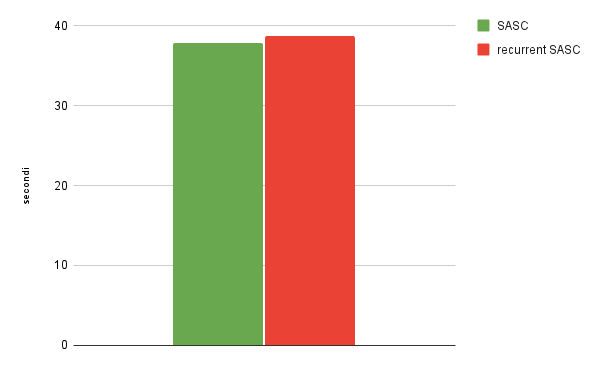
\includegraphics[scale = 0.4]{img/time1.png}
      \caption{}
      \label{img:ista}
    \end{subfigure}
    \begin{subfigure}{0.5\textwidth}
      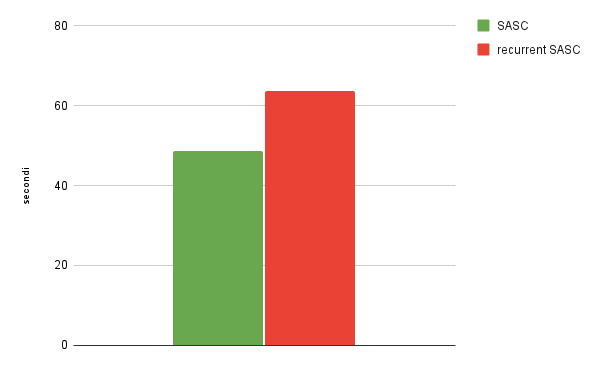
\includegraphics[scale = 0.4]{img/time2.png}
      \caption{}
      \label{img:istb}
    \end{subfigure}
    \caption{Istogrammi relativi allo studio del tempo medio  (espresso in \emph{s}) con $d=5$ e $c=5$, nella figura \ref{img:ista}, e del tempo medio (espresso in \emph{s}) con $d$ e $c$ uguali a  INT\_MAX nella figura \ref{img:istb}}
  \end{figure}

\chapter{Conclusioni}

Per quanto riguarda l'implementazione del recurrent SASC nel linguaggio \textit{C}, si è riusciti a creare un codice che cerchi l'albero che massimizza la likelihood, rispettando le regole di correttezza degli alberi creati ad ogni step, con backmutation e recurrent mutation, come ci si era prefissati.\\\\
Per quanto concerne invece i tempi di esecuzione del codice, visto che non ci si aspetta dati reali con valori di $d$ e $c$ grandi, ci si può ritenere soddisfatti, nonostante le performance scarse quando questi sono molto alti.\\\\
\textit{Concludendo si può dire di aver ottenuto i risultati che erano stati prefissati nel progetto formativo e posso, a titolo personale, ritenermi soddisfatto dell’esperienza}.

\singlespacing
\newpage
\phantomsection
\addcontentsline{toc}{chapter}{Bibliografia e sitografia}
\printbibliography[title={Bibliografia e sitografia}]

\end{document}
